% !TeX root = ../main.tex

\chapter{基于模型的优化}
\label{chap:optimization}
\section{流量预测}
\subsection{离散时间情况}
第\ref{chap:model}章中描述的模型建立在连续时间下。在实际的传输中考虑仅每个比特的情况会更加节省计算的复杂度,因此
在离散的情况下更为合适。
在离散的情况下,式\ref{equ:time}中的$t_i$会按照当前的发送速率转换为每个比特上的ON或OFF状态。比如,延续时间长度为0.1ms的一帧在500kpbs的速率下,就对应50个比特的有状态长度。

为了计算每一比特上对于ON/OFF状态的预测,最直观的方法是利用\emph{整数分解}进行预测。假设即将发送的帧长度为$L$比特,整数分解算法需要找到所有有序$k$元组$(l_1, \cdots, l_k)$,满足
\begin{equation}
	\sum_{i = 1}^{k} l_i = L,
\end{equation}
其中$k,l_i \in \mathbb{Z}^+,\,i = 1,\cdots,k$。每一个$l_i$都代表着当前ON/OFF状态持续的长度(以比特为单位),在给定传输速率$r$的情况下,可以转换为实际长度时间$t_i = \frac{l_i}{r}$。依照经验分布函数,可以得到$l_i$出现的概率
\begin{equation}
p_{l_i} = 
\begin{cases}
f_{ON}^{-1}(l_i), \,i\, mod 2 = 1;\\
f_{OFF}^{-1}(l_i), \,i\, mod 2 = 0
\end{cases}
\end{equation}
那么,对于当前的$k$元组$(l_1, \cdots, l_k)$,出现总概率为$\prod_{i}p_i$。再对所有可能的分解依照出现总概率进行加权,完成预测。

但这种方法的复杂度很高,在第\ref{chap:evaluation}章有具体的评估数据。更适合该模型的方法是利用\emph{蒙特卡罗方法}进行模拟。在单次模拟中,当ON/OFF状态在相互转化时,利用均匀分布和经验累积分布函数按下式进行随机采样得到$l_i$:
\begin{equation}
l_i = \inf_l\{F_{ON/OFF}(l) < u_i\},
\end{equation}
其中$U_i \sim U[0,1]$。在进行$N$此模拟后,对个比特位求平均实现预测。这里记预测后的结果为$(p_1, \cdots, p_L)$,其中$p_i$表示第$i$比特是ON状态的概率。

图\ref{fig:heatmap_256_500_mall}-\ref{fig:heatmap_256_500_lab}展示了不同环境、速率和帧长的情况下,使用蒙特卡罗方法进行500000此模拟的预测结果。图中显示的是每一比特上会是ON状态的概率。总的来看,在实验室和商场中ON状态更容易出现,而家庭环境中几乎都是OFF状态。这与之前的分析是相符合的——在商场和实验室中用户使用网络更加频繁,因此会更容易搭上环境中的流量。另一方面,更高的传输速率和更短的帧长会更容易遇见ON状态,直觉上,符合这两个条件的帧可以在当前环境中的Wi-Fi数据消失之前完成传输。
\begin{figure}[t]
	\begin{minipage}[b]{.32\linewidth}
		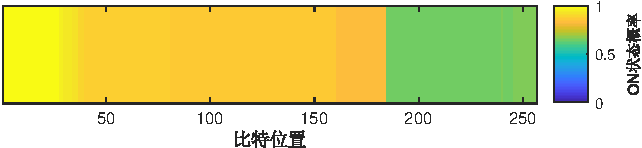
\includegraphics[width = \linewidth]{opt_figure1_256_500_mall-cropped}
		\subcaption{商场环境,256比特,500kbps。}\label{fig:heatmap_256_500_mall}
	\end{minipage}
	\hfill
	\begin{minipage}[b]{.32\linewidth}
		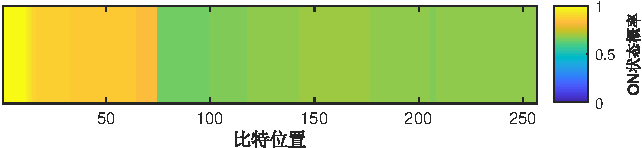
\includegraphics[width = \linewidth]{opt_figure1_256_200_mall-cropped}
		\subcaption{商场环境,256比特,200kbps。}\label{fig:heatmap_256_200_mall}
	\end{minipage}
	\hfill
	\begin{minipage}[b]{.32\linewidth}
		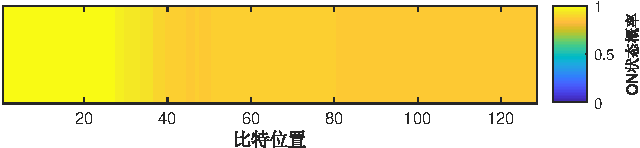
\includegraphics[width = \linewidth]{opt_figure1_128_500_mall-cropped}
		\subcaption{商场环境,128比特,500kbps。}\label{fig:heatmap_128_500_mall}
	\end{minipage}
	
	\begin{minipage}[b]{.32\linewidth}
		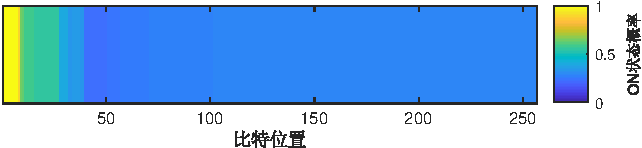
\includegraphics[width = \linewidth]{opt_figure1_256_500_home-cropped}
		\subcaption{家庭环境,256比特,500kbps。}\label{fig:heatmap_256_500_home}
	\end{minipage}
	\hfill
	\begin{minipage}[b]{.32\linewidth}
		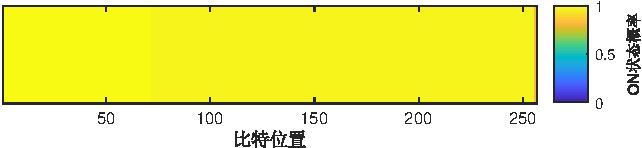
\includegraphics[width = \linewidth]{opt_figure1_256_500_lab-cropped}
		\subcaption{实验室环境,256比特,500kbps。}\label{fig:heatmap_256_500_lab}
	\end{minipage}
	\hfill
	\begin{minipage}[b]{.32\linewidth}
		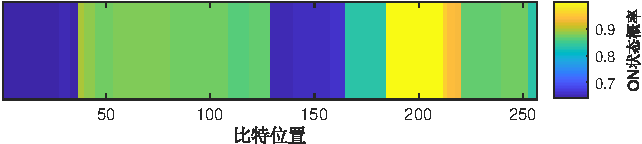
\includegraphics[width = \linewidth]{opt_figure2_256_500_lab_deperm-cropped}
		\subcaption{热力图(\subref{fig:heatmap_256_500_mall})置换后。}\label{fig:heatmap_perm}
	\end{minipage}
	\caption{不同环境、不同帧长、不同传输速率下的预测热力图。(\subref{fig:heatmap_perm})展示了置换的效果。}\label{fig:heatmap}
\end{figure}

\subsection{预测对LDPC解码的影响}

LDPC的解码使用信念传播算法(Belief propagation),也称为信息传递算法(Message-passing)。对于传输的LDPC码字$c = (c_1, c_2, …, c_{L})$,LDPC解码算法的输入是对数似然比(Log-likelihood ratio, LLR):
\begin{equation}
\label{equ:llr}
L(c_i)=\log\left(\frac{Pr(c_i=0|channel\,output\,for\,c_i)}{Pr(c_i=1|channel\,output\,for \,c_i)}\right)
\end{equation}
在算法回一句初始LLR不断更新迭代,更新对每一个比特$c_i$的LLR估计。在算法中,传输信息的比特和负责校验的比特之间会相互交换LLR信息,这也是算法名称的由来。

值得注意的是,初始LLR的计算是需要对信道的先验的。如果简单的考虑为加性高斯信道,会导致LDPC解码的效果很差;而结合对信道的先验的情况下,式\ref{equ:llr}可以写为:
\begin{equation}
\label{equ:llr_new}
L(c_i)=\log\left(\frac{ p_i \frac{1}{1+ratio_i} + \frac{1}{2} (1-p_i) }{ p_i \frac{1}{1+1/ratio_i} + \frac{1}{2} (1-p_i)  }\right),
\end{equation}
其中$ratio_i = Pr\{c_i$信道输出$|c_i=1\}/Pr\{c_i$信道输出$|c_i=0\}$。
\section{根据预测优化}

\subsection{置换}
\label{subsec:perm}
在针对每一比特的预测概率基础上,可以引入交织(置换)机制使得帧可以以更高的概率应对突发错误,以提高系统的可靠性。对于长度为$L$比特的帧$F$,假设当前使用的是$(n,k)$的码,
%\footnote{如果使用里德-所罗门码也是相似的,将长度$L$换为$L/8$即可}。
通常情况下,$L$都是可以被$n$整除的,不足的部分也可以通过填充实现。假设$L = bn$,那么在编码过程中会对原始数据分成$b$块。由于我们已知每一比特遇到OFF状态的概率,可以通过\emph{将高概率出现OFF状态的位置均匀置换到每一块中}。

寻找一个置换$\sigma^\ast$,使得
\begin{equation}
\sigma^\ast = \max_\sigma \Var \{ (z_1, \cdots, z_b) \} 
\end{equation}
其中$z_i, i = 1,\cdots,b$是置换后的帧$sigma(F)$每$i$块中可能出现OFF的个数。由于预测给出的是概率值,因此我们会设置一个阈值,概率小于阈值的会被认定为OFF。图\ref{fig:heatmap_perm}展示了对图\ref{fig:heatmap_256_500_mall}进行置换后的热力图,集中在第二块中的易遇见错误的比特会被均匀分散到两块中,从而提升可靠性。

\subsection{动态参数调节}

在采用不同的帧长和传输率的情况下,即便是基于相同的累积分布函数,也会产生不同的预测效果。
%一般来说,在帧长一定的情况下,选择越高的传输率由越高的机会在ON状态下发送完数据;在传输率一定的情况下,选择越长的帧长会有更高的可能性再发送的过程中遇见OFF状态,但是会有更高的吞吐量。同样,对环境的预测也会影响码率的选择:如果预测环境中Wi-Fi流量比较繁忙,那么可以提升码率,以达到更高的吞吐量;如果预测环境中会出现较多的OFF状态,会选择降低码率,已保证该帧可以正确传输。
具体来讲,假设当前使用的编码在每一块中可以纠正$t$比特错误,在最理想的情况下,结合置换一共可以纠正$bt$比特的错误。将最有可能出现OFF状态的$bt$比特利用码进行纠正,剩下所有比特位置全部为ON状态的概率可以由下式计算:
\begin{equation}
p_{success} = \prod_{i = bt+1}^{L} p_i^{'},
\end{equation}
其中$p_i^{'}$是对原有预测升序排列后的概率。为了平衡长度的因素,实际中$p_{success}$选择的是所有需计算的概率的集合均值$p_{success, GM}$。进一步,在给定帧长、传输率和码率的选择范围下,我们求解下式的最优化问题:
\begin{equation}
\label{equ:dynamic_parameter}
fLen^\ast, dr^\ast, cr^\ast = \max_{fLen, dr, cr} \frac{p_{success, GM}\cdot cr}{fLen\cdot dr},
\end{equation}
其中$fLen,dr,cr$依次指帧长、传输率和码率。本质上,式\ref{equ:dynamic_parameter}是在求解单位时间内可以正确传输的比特数。由于$p_{success}p_{success, GM}$一般会很小,因此采用对数形式的式\ref{equ:dynamic_parameter}。